\documentclass[tikz,border=6mm]{standalone}
\usepackage{tikz}
\usepackage{xcolor}
\usetikzlibrary{arrows.meta,calc,decorations.pathmorphing,decorations.markings,shapes.geometric,positioning,backgrounds,fit,shadings,patterns}
\definecolor{substblue}{RGB}{70,130,180}
\definecolor{procamber}{RGB}{180,110,30}
\definecolor{feltgreen}{RGB}{0,110,55}
\definecolor{bgcream}{RGB}{252,248,240}
\definecolor{atomblue}{RGB}{100,160,210}
\definecolor{emphred}{RGB}{160,40,0}
\definecolor{panelborder}{RGB}{180,170,155}

\begin{document}
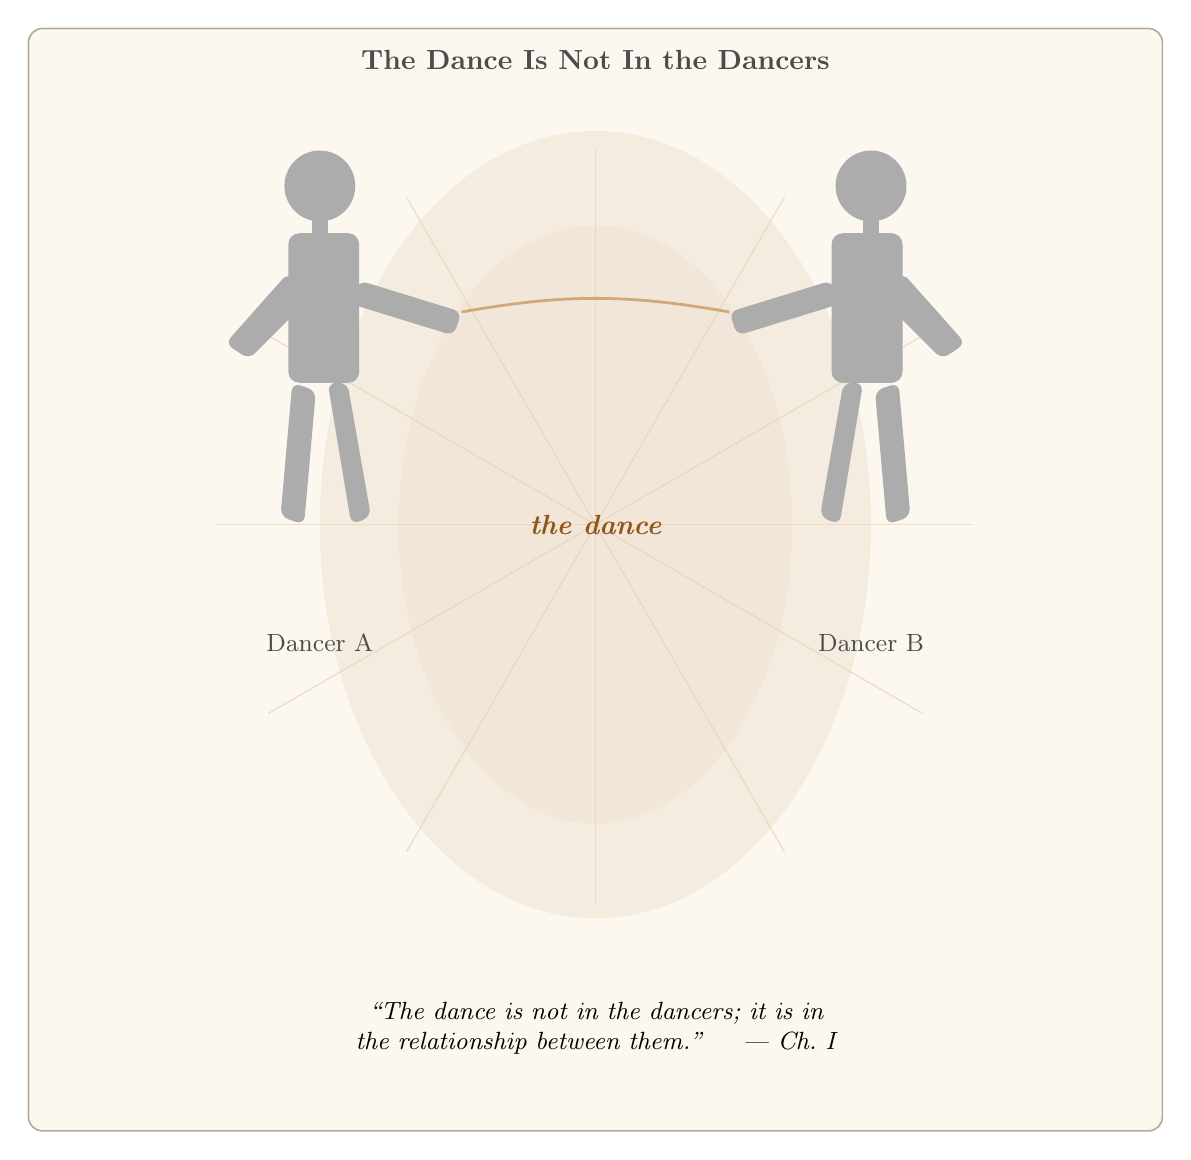
\begin{tikzpicture}[>=Stealth,font=\small]

%% ── background ───────────────────────────────────────────────────────────────
\fill[bgcream,rounded corners=5pt] (-2.2,-6.5) rectangle (12.2,7.5);
\draw[panelborder,rounded corners=5pt,line width=0.6pt]
  (-2.2,-6.5) rectangle (12.2,7.5);

%% ── title ────────────────────────────────────────────────────────────────────
\node[font=\normalsize\bfseries,gray!60!black] at (5.0,7.1)
  {The Dance Is Not In the Dancers};

%% ════════════════════════════════════════════════════════════════════════════
%%  RELATIONAL GLOW — warm ellipse in centre, drawn first (behind dancers)
%% ════════════════════════════════════════════════════════════════════════════
\begin{scope}
  \clip (-2.2,-6.5) rectangle (12.2,7.5);
  \fill[procamber!25,opacity=0.9] (5.0,1.2) ellipse (2.5cm and 3.8cm);
  \fill[procamber!15,opacity=0.8] (5.0,1.2) ellipse (3.5cm and 5.0cm);
\end{scope}

%% radiating spoke lines from the relational centre
\foreach \ang in {0,30,...,330}{%
  \draw[procamber!30,line width=0.5pt,opacity=0.7]
    (5.0,1.2) -- ++(\ang:4.8cm);
}

%% ════════════════════════════════════════════════════════════════════════════
%%  LEFT DANCER — simplified silhouette, facing right
%%  Origin of dancer body: (1.5, 1.0)
%% ════════════════════════════════════════════════════════════════════════════
\begin{scope}[shift={(1.5,1.0)}]
  %% head
  \fill[gray!65] (0,4.5) circle (0.45cm);
  %% neck
  \fill[gray!65] (-0.1,3.9) rectangle (0.1,4.1);
  %% torso
  \fill[gray!65,rounded corners=4pt]
    (-0.4,2.0) -- (-0.4,3.9) -- (0.5,3.9) -- (0.5,2.0) -- cycle;
  %% left arm (extends leftward/back)
  \fill[gray!65,rounded corners=3pt]
    (-0.4,3.4) -- (-1.2,2.5) -- (-0.9,2.3) -- (-0.1,3.1) -- cycle;
  %% right arm (reaches toward centre/partner)
  \fill[gray!65,rounded corners=3pt]
    (0.5,3.3) -- (1.8,2.9) -- (1.7,2.6) -- (0.4,3.0) -- cycle;
  %% left leg
  \fill[gray!65,rounded corners=3pt]
    (-0.35,2.0) -- (-0.5,0.3) -- (-0.2,0.2) -- (-0.05,1.9) -- cycle;
  %% right leg (slight step)
  \fill[gray!65,rounded corners=3pt]
    (0.1,2.0) -- (0.4,0.2) -- (0.65,0.3) -- (0.35,2.0) -- cycle;
\end{scope}

%% ════════════════════════════════════════════════════════════════════════════
%%  RIGHT DANCER — mirror silhouette, facing left
%%  Origin of dancer body: (8.5, 1.0)
%% ════════════════════════════════════════════════════════════════════════════
\begin{scope}[shift={(8.5,1.0)},xscale=-1]
  %% head
  \fill[gray!65] (0,4.5) circle (0.45cm);
  %% neck
  \fill[gray!65] (-0.1,3.9) rectangle (0.1,4.1);
  %% torso
  \fill[gray!65,rounded corners=4pt]
    (-0.4,2.0) -- (-0.4,3.9) -- (0.5,3.9) -- (0.5,2.0) -- cycle;
  %% back arm
  \fill[gray!65,rounded corners=3pt]
    (-0.4,3.4) -- (-1.2,2.5) -- (-0.9,2.3) -- (-0.1,3.1) -- cycle;
  %% reach arm (toward centre)
  \fill[gray!65,rounded corners=3pt]
    (0.5,3.3) -- (1.8,2.9) -- (1.7,2.6) -- (0.4,3.0) -- cycle;
  %% left leg
  \fill[gray!65,rounded corners=3pt]
    (-0.35,2.0) -- (-0.5,0.3) -- (-0.2,0.2) -- (-0.05,1.9) -- cycle;
  %% right leg (slight step)
  \fill[gray!65,rounded corners=3pt]
    (0.1,2.0) -- (0.4,0.2) -- (0.65,0.3) -- (0.35,2.0) -- cycle;
\end{scope}

%% ── connecting arm curves ─────────────────────────────────────────────────
%% Hands of left dancer end near (3.3, 3.9), right dancer near (6.7, 3.9)
\draw[procamber!60,line width=1.0pt,bend left=10]
  (3.3,3.9) to[out=10,in=170] (6.7,3.9);

%% ════════════════════════════════════════════════════════════════════════════
%%  THE DANCE LABEL — in the relational glow centre
%% ════════════════════════════════════════════════════════════════════════════
\node[font=\normalsize\bfseries\itshape,procamber!80!black,align=center]
  at (5.0,1.2) {the dance};

%% ── dancer labels ────────────────────────────────────────────────────────────
\node[font=\small,gray!60!black] at (1.5,-0.3) {Dancer A};
\node[font=\small,gray!60!black] at (8.5,-0.3) {Dancer B};

%% ── caption ──────────────────────────────────────────────────────────────────
\node[font=\small\itshape,text width=11cm,align=center]
  at (5.0,-5.2)
  {``The dance is not in the dancers; it is in the relationship between them.''
   \quad --- Ch.~I};

\end{tikzpicture}
\end{document}
